\documentclass[11pt,compress,t,notes=noshow, aspectratio=169, xcolor=table]{beamer}

\usepackage{../../style/lmu-lecture}
% Defines macros and environments
% This file is included in slides and exercises

% Rarely used fontstyle for R packages, used only in 
% - forests/slides-forests-benchmark.tex
% - exercises/single-exercises/methods_l_1.Rnw
% - slides/cart/attic/slides_extra_trees.Rnw
\newcommand{\pkg}[1]{{\fontseries{b}\selectfont #1}}

% Spacing helpers, used often (mostly in exercises for \dlz)
\newcommand{\lz}{\vspace{0.5cm}} % vertical space (used often in slides)
\newcommand{\dlz}{\vspace{1cm}}  % double vertical space (used often in exercises, never in slides)
\newcommand{\oneliner}[1] % Oneliner for important statements, used e.g. in iml, algods
{\begin{block}{}\begin{center}\begin{Large}#1\end{Large}\end{center}\end{block}}

% Don't know if this is used or needed, remove?
% textcolor that works in mathmode
% https://tex.stackexchange.com/a/261480
% Used e.g. in forests/slides-forests-bagging.tex
% [...] \textcolor{blue}{\tfrac{1}{M}\sum^M_{m} [...]
% \makeatletter
% \renewcommand*{\@textcolor}[3]{%
%   \protect\leavevmode
%   \begingroup
%     \color#1{#2}#3%
%   \endgroup
% }
% \makeatother




\title{Interpretable Machine Learning}
% \author{LMU}
%\institute{\href{https://compstat-lmu.github.io/lecture_iml/}{compstat-lmu.github.io/lecture\_iml}}
\date{}

%\bibliography{feature-importance}
%\usepackage{Sweave}
\begin{document}
	\newcommand{\titlefigure}{figure_man/feature-importance.png}
    \newcommand{\learninggoals}{
    	\item Understand how PFI is computed
    	\item Understanding strengths and weaknesses}
	% Set style/preamble.Rnw as parent.
	
	% Load all R packages and set up knitr
	
	% This file loads R packages, configures knitr options and sets preamble.Rnw as 
	% parent file
	% IF YOU MODIFY THIS, PLZ ALSO MODIFY setup.Rmd ACCORDINGLY...
	
	% Defines macros and environments

	\lecturechapter{Permutation Feature Importance (PFI)}
	\lecture{Interpretable Machine Learning}
	
	% ------------------------------------------------------------------------------

% \begin{frame}{Permutation Feature Importance Idea \citebutton{Breiman (2001)}{https://doi.org/10.1023/A:1010933404324}}

% In general, feature importance methods share two components
% \lz
% \begin{enumerate}
%   \item \textbf{Perturbation/Removal:} Generate predictions for which the feature of interest has been perturbed or removed.
%   \item \textbf{Performance Comparison:} Compare performance under perturbation/removal with the original model performance.
% \end{enumerate}
% \lz
% \textbf{Permutation Feature Importance Idea:} "Remove" the feature of interest $x_j$ by perturbing it such that it is uninformative. Therefore, resample the variable from its marginal distribution $\P(x_j)$, e.g. by randomly permuting observations in $x_j$.

% %\footnote[frame]{\fullcite{Breiman2001rf}}

% %\framebreak

% %\begin{figure}
% %  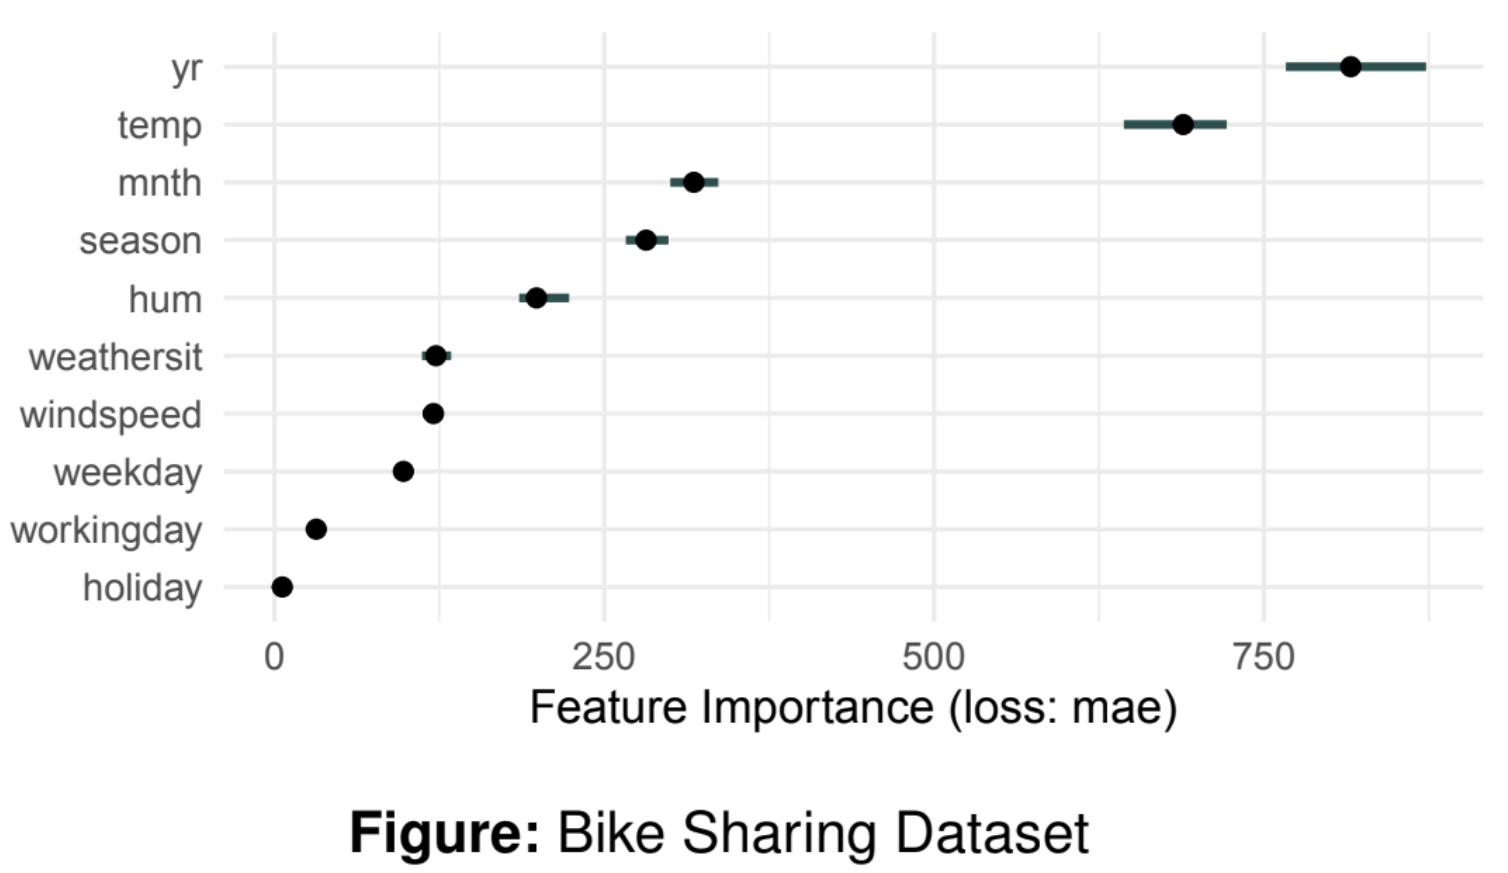
\includegraphics[width=0.75\textwidth]{figure_man/feature-importance.png}
% %\end{figure}

% %\vspace{-0.2cm}
% %\tiny{Fisher et al. (2018). All models are wrong but many are useful: Variable importance for black-box, proprietary, or misspecified prediction models, using model class reliance. arXiv preprint arXiv:1801.01489 (2018).}

% \end{frame}

\begin{frame}{Permutation Feature Importance (PFI) \citebutton{Breiman (2001)}{https://doi.org/10.1023/A:1010933404324}}


% TODO: explain this idea better in one separate slide, e.g. we have a fixed model we want to analyze and a data set. Our aim is to understand the importance of features. We would like to remove a feature and measure its "added value" w.r.t. performance compared to not removing it. But we cannot remove it as the model is fixed and was already trained with that feature -> permuting is the next best thing we can do to "destroy" the information of the feature -> another possibility could be to add some noise to the feature to perturb it but this would change the marginal distribution

\textbf{Idea:} "Destroy" feat. of interest $x_j$ by perturbing it s.t. it becomes uninformative, e.g., randomly permute obs. in $x_j$ (marginal distribution $\P(x_j)$ stays the same).  %Therefore, resample the variable from its marginal distribution $\P(x_j)$, e.g. by randomly permuting observations in $x_j$.

PFI for features $x_S$ using test data $\D$:
\begin{itemize}
  \item Measure the error {\color{blue}\textbf{without permuting feat.}} and {\color{red}\textbf{with permuted feat. values}} $\pert{x}{}{}_S$
  \item Repeat permuting the feat. (e.g., $m$ times) and avg. the difference of both errors: 
\begin{align*}
&\widehat{PFI}_S = \tfrac{1}{m} \textstyle\sum\nolimits_{k = 1}^{m} \riske (\fh, {\color{red}\pert{\D}{S}{}_{(k)}}) - \riske (\fh, {\color{blue}\D}),\\&\text{ where }
\riske(\fh, \D) = \frac{1}{n} \sum\nolimits_{(x, y) \in \D}  L(\fh(x), y)
\end{align*}
\end{itemize}
\pause
The data $\D$ where $x_S$ is replaced with $\pert{x}{S}{}$ is denoted as $\pert{\D}{S}{}$.\\
Example of permuting feature $x_S$ with $S = \{1\}$ and $m=6$:

% TODO: update to new notation
\begin{center}
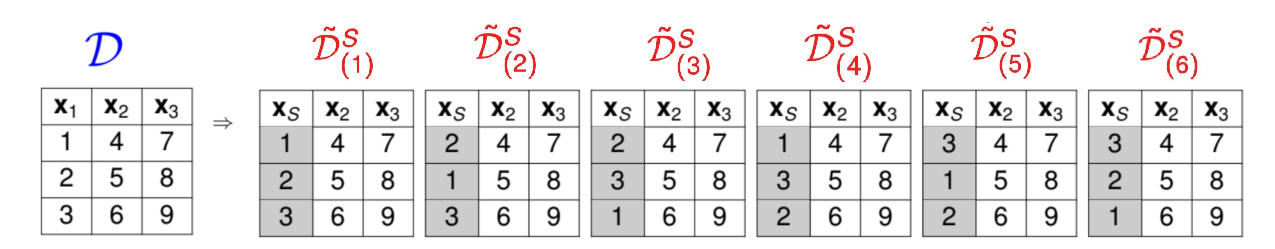
\includegraphics[width=0.75\textwidth]{figure_man/permuted-fv.pdf}
\end{center}

\vspace*{0.2cm}
{\scriptsize{Note: 
The $S$ in $x_S$ refers to a \textbf{S}ubset of features for which we are interested in their effect on the prediction.\\
Here: We calculate the feature importance for one feature at a time $|S| = 1$.}\par}

\end{frame}



% \begin{columns, totalwidth=\textwidth}
%   \begin{column}{0.5\textwidth}
%     \only<1-3,5-7>{$\hspace{36pt}{\color{white}\riske(\fh, {\color{red}\pert{\D}{S}{}_{(k)}}) - \riske(\fh, {\color{blue}\D})}$}
%   \only<4>{$\hspace{36pt}\riske(\fh, {\color{red}\pert{\D}{S}{}_{(k)}}) - \riske(\fh, {\color{blue}\D}),$ where 
% $\riske(\fh, \D) =$ \scalebox{0.7}{$\frac{1}{n} \sum\nolimits_{(x, y) \in \D}$} $\scriptstyle L(\fh(x), y)$}
% % $\scriptstyle\riske(\fh, \D) =$ \scalebox{0.7}{$\frac{1}{n} \sum\nolimits_{(x, y) \in \D}$} $\scriptstyle L(\fh(x), y)$}
% %   \only<5-6>{$\hspace{36pt}{\color{white}\riske(\fh, {\color{red}\pert{\D}{S}{}_{(k)}}) - \riske(\fh, {\color{blue}\D})}$}
  
%   \begin{center}
%   \only<1>{\includegraphics[page=2, trim=0pt 5pt 0 66pt, clip, width=\textwidth]{figure_man/pfi_demo2}}%
%   \only<2>{\includegraphics[page=3, trim=0pt 5pt 0 66pt, clip, width=\textwidth]{figure_man/pfi_demo2}}%
%   \only<3-4>{\includegraphics[page=4, trim=0pt 5pt 0 66pt, clip, width=\textwidth]{figure_man/pfi_demo2}}%
%   \only<5>{\includegraphics[page=5, trim=0pt 5pt 0 66pt, clip, width=\textwidth]{figure_man/pfi_demo2}}%
%   \only<6>{\includegraphics[page=6, trim=0pt 5pt 0 66pt, clip, width=\textwidth]{figure_man/pfi_demo2}}%
%   \only<7>{\includegraphics[page=7, trim=0pt 5pt 0 66pt, clip, width=\textwidth]{figure_man/pfi_demo2}}%
%   \end{center}
%   \end{column}
%   \begin{column}{0.5\textwidth}
  
%   \begin{itemize}
%     \only<1-2>{\item[1.]\textbf{Perturbation:} Sample feature values from the distribution of $x_S$ ($P(X_S)$). \newline $\Rightarrow$ Randomly permute feature $x_S$. Replace the original feature with the permuted feature $\pert{x}{}{}_S$ and create data with permuted feature   $\pert{\D}{S}{}$.}
%     \only<2>{\item[2.] \textbf{Prediction:} Make predictions for both data, i.e., $\D$ and $\pert{\D}{S}{}$.}
%     \only<3-4>{\item[3.] \textbf{Aggregation:}
%       \begin{itemize}
%         \item Compute the loss for each observation in both data sets.
%       \end{itemize}}
%     \only<5>{\item[3.] \textbf{Aggregation:}
%       \begin{itemize}
%         \item Compute the loss for each observation in both data sets.
%       \item Take the difference of both losses $\Delta L$ for each observation.
%       \end{itemize}}
%      \only<6>{\item[3.] \textbf{Aggregation:}
%       \begin{itemize}
%         \item Compute the loss for each observation in both data sets.
%         \item Take the difference of both losses $\Delta L$ for each observation.
%         \item Average this change in loss across all observations.
%       \end{itemize}}
%     \only<7>{\item[3.] \textbf{Aggregation:}
%       \begin{itemize}
%         \item Compute the loss for each observation in both data sets.
%         \item Take the difference of both losses $\Delta L$ for each observation.
%         \item Average this change in loss across all observations.
%         \item Also, average over multiple repetitions, if available.
%       \end{itemize}}
%   \end{itemize}
%   \end{column}
% \end{columns}



\begin{frame}{Permutation Feature Importance}

  \only<1-4>{$\hspace{80pt}{\color{white}\riske(\fh, {\color{red}\pert{\D}{S}{}_{(k)}}) - \riske(\fh, {\color{blue}\D})}$}%
  \only<5-6>{$\hspace{80pt}\riske(\fh, {\color{red}\pert{\D}{S}{}_{(k)}}) - \riske(\fh, {\color{blue}\D})$}%
% $\scriptstyle\riske(\fh, \D) =$ \scalebox{0.7}{$\frac{1}{n} \sum\nolimits_{(x, y) \in \D}$} $\scriptstyle L(\fh(x), y)$}
%   \only<5-6>{$\hspace{36pt}{\color{white}\riske(\fh, {\color{red}\pert{\D}{S}{}_{(k)}}) - \riske(\fh, {\color{blue}\D})}$}
  
  \begin{center}
  \only<1>{\includegraphics[page=2, trim=0pt 5pt 0 66pt, clip, width=0.7\textwidth]{figure_man/pfi_demo2}}%
  \only<2>{\includegraphics[page=3, trim=0pt 5pt 0 66pt, clip, width=0.7\textwidth]{figure_man/pfi_demo2}}%
  \only<3>{\includegraphics[page=4, trim=0pt 5pt 0 66pt, clip, width=0.7\textwidth]{figure_man/pfi_demo2}}%
  \only<4>{\includegraphics[page=5, trim=0pt 5pt 0 66pt, clip, width=0.7\textwidth]{figure_man/pfi_demo2}}%
  \only<5>{\includegraphics[page=6, trim=0pt 5pt 0 66pt, clip, width=0.7\textwidth]{figure_man/pfi_demo2}}%
  \only<6>{\includegraphics[page=7, trim=0pt 5pt 0 66pt, clip, width=0.7\textwidth]{figure_man/pfi_demo2}}%
  \end{center}
  
  \begin{itemize}
    \only<1-2>{\item[1.]\textbf{Perturbation:} Sample feature values from the distribution of $x_S$ ($P(X_S)$). \newline 
    $\Rightarrow$ Randomly permute feature $x_S$ \\
    $\Rightarrow$ Replace original feature with permuted feature $\pert{x}{}{}_S$ and create data $\pert{\D}{S}{}$ containing $\pert{x}{}{}_S$}%
    \only<2>{\item[2.] \textbf{Prediction:} Make predictions for both data, i.e., $\D$ and $\pert{\D}{S}{}$}%
    \only<3->{\item[3.] \textbf{Aggregation:}}%
      \begin{itemize}
        \item<3-> Compute the loss for each observation in both data sets%
        \item<4-> Take the difference of both losses $\Delta L$ for each observation%
        \item<5-> Average this change in loss across all observations%
        \only<5>{\\ Note: This is equivalent to computing $\riske$ on both data sets and taking the difference}%
        \item<6-> Repeat perturbation and average over multiple repetitions%
      \end{itemize}
    % \only<3-4>{\item[3.] \textbf{Aggregation:}
    %   \begin{itemize}
    %     \item Compute the loss for each observation in both data sets.
    %   \end{itemize}}
    % \only<5>{\item[3.] \textbf{Aggregation:}
    %   \begin{itemize}
    %     \item Compute the loss for each observation in both data sets.
    %   \item Take the difference of both losses $\Delta L$ for each observation.
    %   \end{itemize}}
    %  \only<6>{\item[3.] \textbf{Aggregation:}
    %   \begin{itemize}
    %     \item Compute the loss for each observation in both data sets.
    %     \item Take the difference of both losses $\Delta L$ for each observation.
    %     \item Average this change in loss across all observations.
    %   \end{itemize}}
    % \only<7>{\item[3.] \textbf{Aggregation:}
    %   \begin{itemize}
    %     \item Compute the loss for each observation in both data sets.
    %     \item Take the difference of both losses $\Delta L$ for each observation.
    %     \item Average this change in loss across all observations.
    %     \item Also, average over multiple repetitions, if available.
    %   \end{itemize}}
  \end{itemize}
\end{frame}

\begin{frame}{Example: Bike Sharing Dataset}

\begin{center}
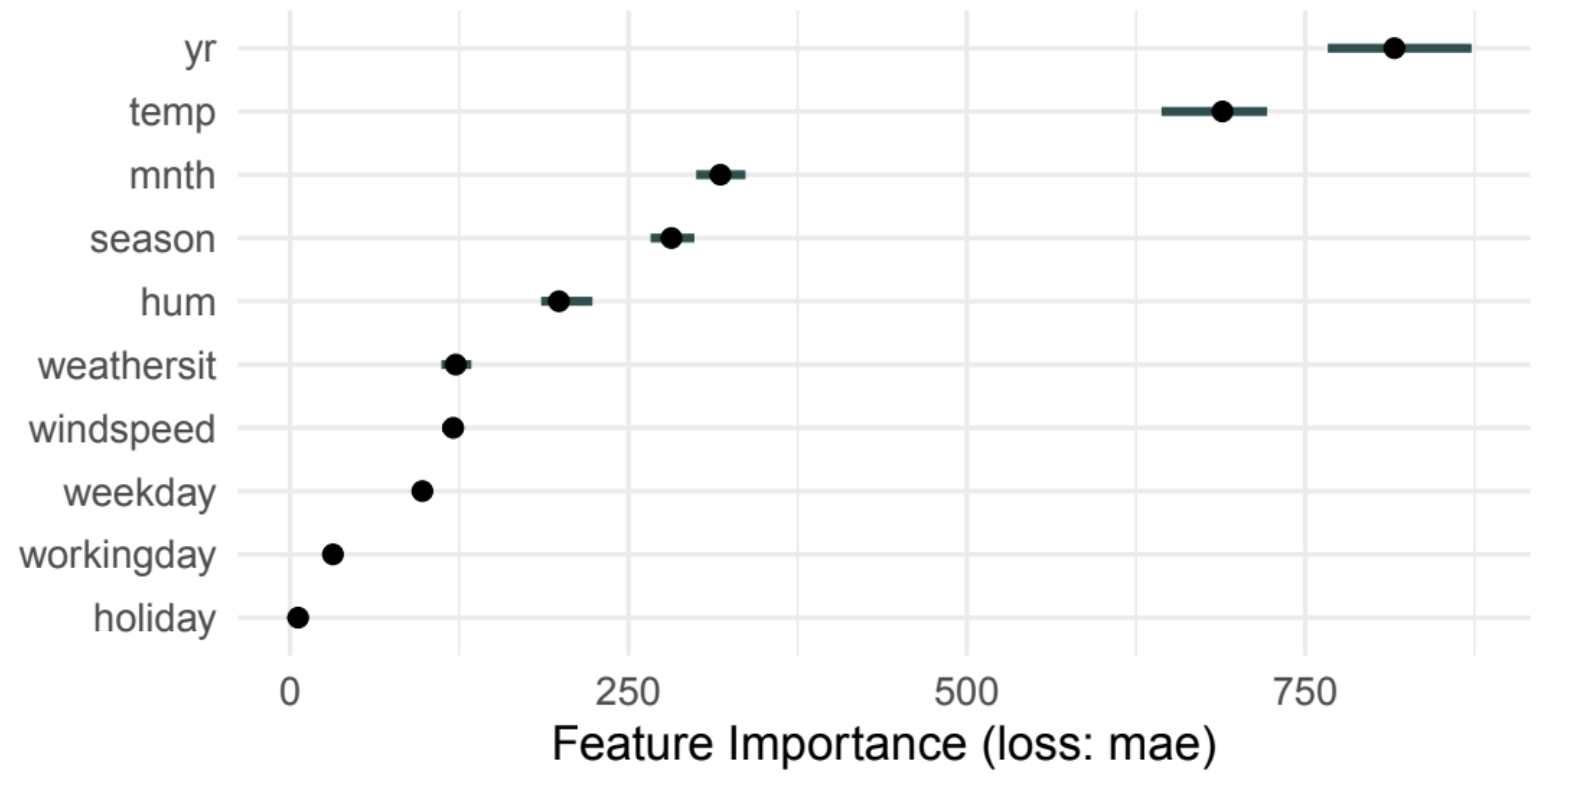
\includegraphics[width=0.6\textwidth]{figure_man/bike-sharing02.png}
\end{center}

\textbf{Interpretation:}

\begin{itemize}
 \item Year (\code{yr}) and Temperature (temp) are most important features
 %Features such as weekday also contribute to the performance.
 \item Destroying information about \code{yr} by permuting it increases mean absolute error of model by 816
 \item $5 \%$ and $95 \%$ quantile of repetitions due multiple permutations are shown as error bars
\end{itemize}
\end{frame}

\begin{frame}{Comments on PFI}
 \begin{itemize}[<+->]
 \itemsep1em
  \item Interpretation: Increase in error when feature's information is destroyed
  \item Results can be unreliable due to random permutations \\
  $\Rightarrow$ Solution: Average results over multiple repetitions
  \item Permuting features despite correlation with other features can lead to unrealistic combinations of feature values (since $\P(x_j,x_{-j}) \neq \P(x_j) \P(x_{-j})$)\\
  $\leadsto$ Extrapolation issue
  \item PFI automatically includes importance of interaction effects with other features \\
  $\Rightarrow$ Permuting $x_j$ also destroys interactions with permuted feature\\
  $\Rightarrow$ PFI score contains importance of all interactions with permuted feature %Not only importance of permuted feature is contained but also importance of all interactions with that feature
  \item Interpretation of PFI depends on whether training or test data is used
 \end{itemize}
\end{frame}

%TODO: Simplify example
\begin{frame}{Comments on PFI - Extrapolation}
 
% %\textbf{Example:} Let $y = x_3 + \epsilon_y$ with $\epsilon_y \sim N(0, 0.1)$ where $x_1$, $x_2 := x_1 + \epsilon_1$ are highly correlated ($x_1 \sim N(0,1), \epsilon_1 \sim N(0, 0.01)$). Let $x_3, x_4 \sim N(0,1)$ be noisy features are independent.
 
%  \textbf{Example:} Let $y = x_3 + \epsilon_y$ with $\epsilon_y \sim N(0, 0.1)$ where $x_1 :=  \epsilon_1$, $x_2 := x_1 + \epsilon_2$ are highly correlated ($\epsilon_1 \sim N(0,1), \epsilon_2 \sim N(0, 0.01)$) and $x_3 := \epsilon_3$, $x_4 := \epsilon_4$,  with $\epsilon_3, \epsilon_4 \sim N(0,1)$. All noise terms are independent.
%  Fitting a LM yields $\fh(\xv) \approx 0.3 x_1 - 0.3 x_2 + x_3$.
% \pause

% %\begin{figure}
% % \hfill
% %   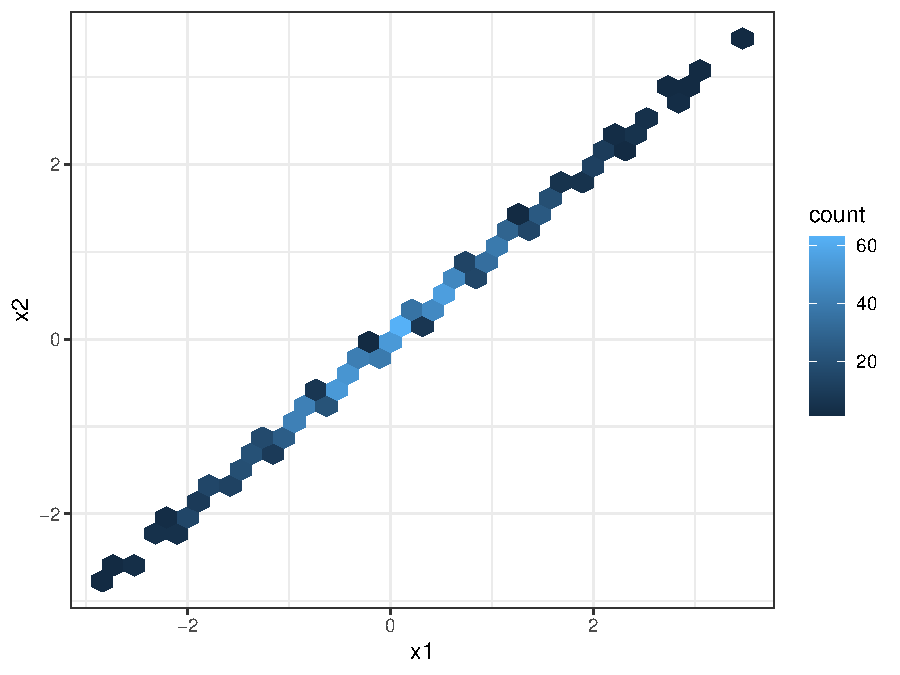
\includegraphics[width=0.3\linewidth]{figure_man/pfi_hexbin_pre.pdf}\hfill
% %   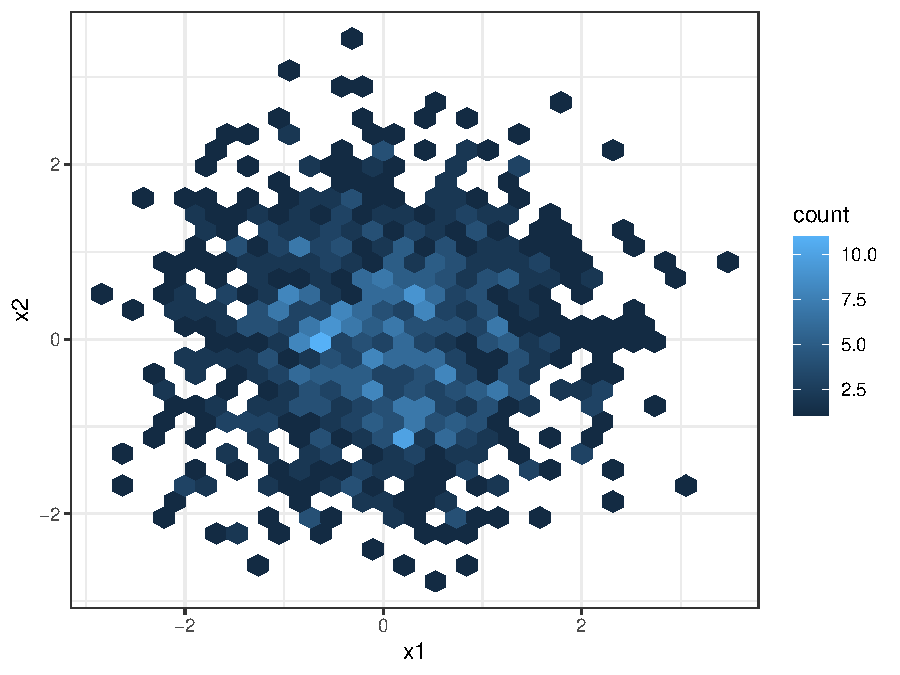
\includegraphics[width=0.3\linewidth]{figure_man/pfi_hexbin_post.pdf} \hfill
% %   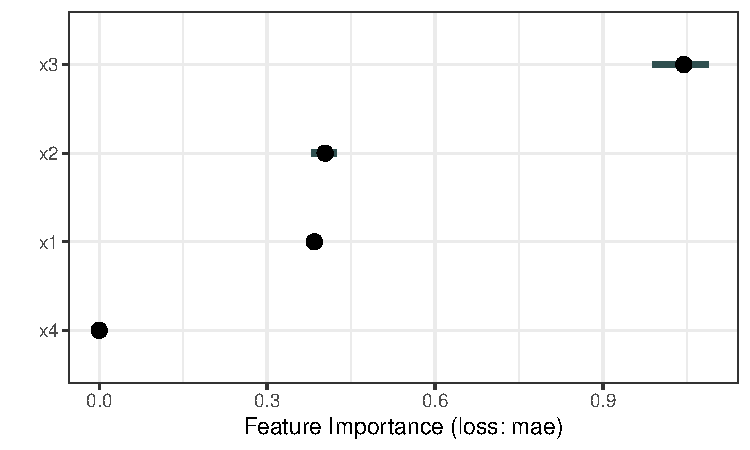
\includegraphics[width=0.39\linewidth]{figure_man/pfi_extrapolation.pdf} \hfill
% \centerline{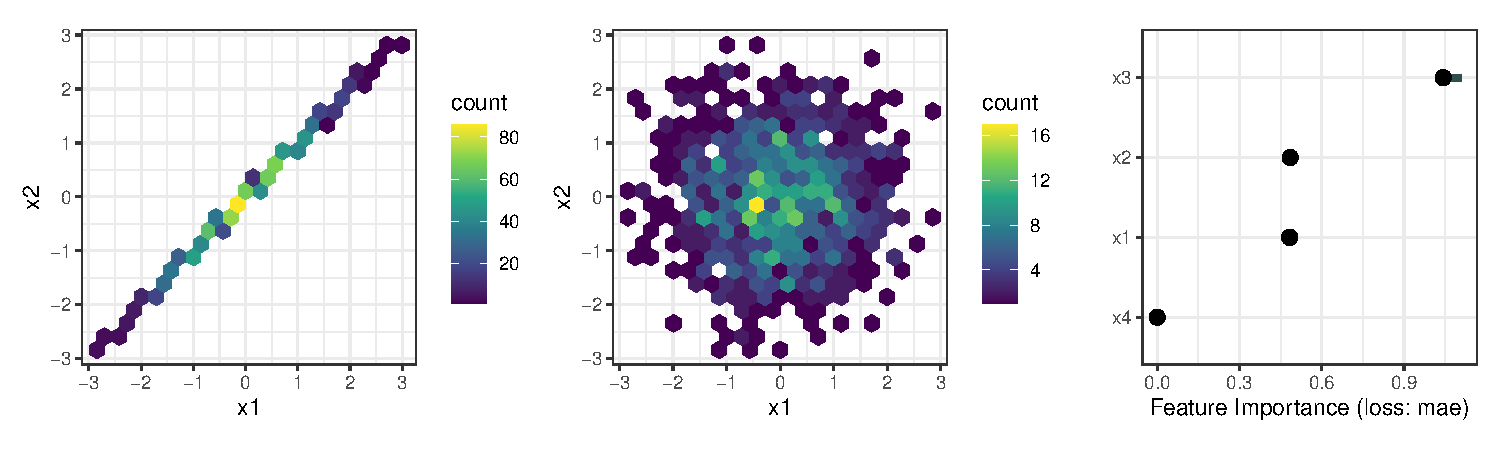
\includegraphics[width=0.9\linewidth]{figure_man/pfi_hexbin_extrapolation.pdf}}
% Hexbin plot of $x_1, x_2$ before permuting $x_1$ (left), after permuting $x_1$ (center), and PFI scores (right)
% \\
% \pause
% % \caption{Density plot for $x_1, x_2$ before permuting $x_1$ (left) and after permuting $x_1$ (center). Right: PFI including $.05$ to $.95$ quantiles.}
% %\end{figure}
% % 
% $\Rightarrow$ $x_1$ and $x_2$ should be irrelevant for the prediction $\fh(\xv)$ %for $\{\xv: \P(\xv) > 0\}$ 
% since $0.3 x_1 - 0.3 x_2 \approx 0$ \\
% $\Rightarrow$ PFI evaluates model on unrealistic obs. outside $\P(\xv)$ $\leadsto$ $x_1$, $x_2$ are considered relevant (PFI $> 0$)
% %$\Rightarrow$ Since PFI evaluates the model on unrealistic observations, the features $x_1$ and $x_2$ are nevertheless considered relevant


\textbf{Example:} Let $y = x_3 + \epsilon_y$, with $\epsilon_y \sim \mathcal{N}(0, 0.1)$.

\begin{itemize}
  \item $x_1 := \epsilon_1$, $x_2 := x_1 + \epsilon_2$ are highly correlated  
        ($\epsilon_1 \sim \mathcal{N}(0,1)$, $\epsilon_2 \sim \mathcal{N}(0, 0.01)$)
  \item $x_3 := \epsilon_3$, $x_4 := \epsilon_4$, with $\epsilon_3, \epsilon_4 \sim \mathcal{N}(0,1)$
  \item All noise terms are independent
\end{itemize}

Fitting a linear model yields $\hat{f}(\xv) \approx 0.3 x_1 - 0.3 x_2 + x_3$

\centerline{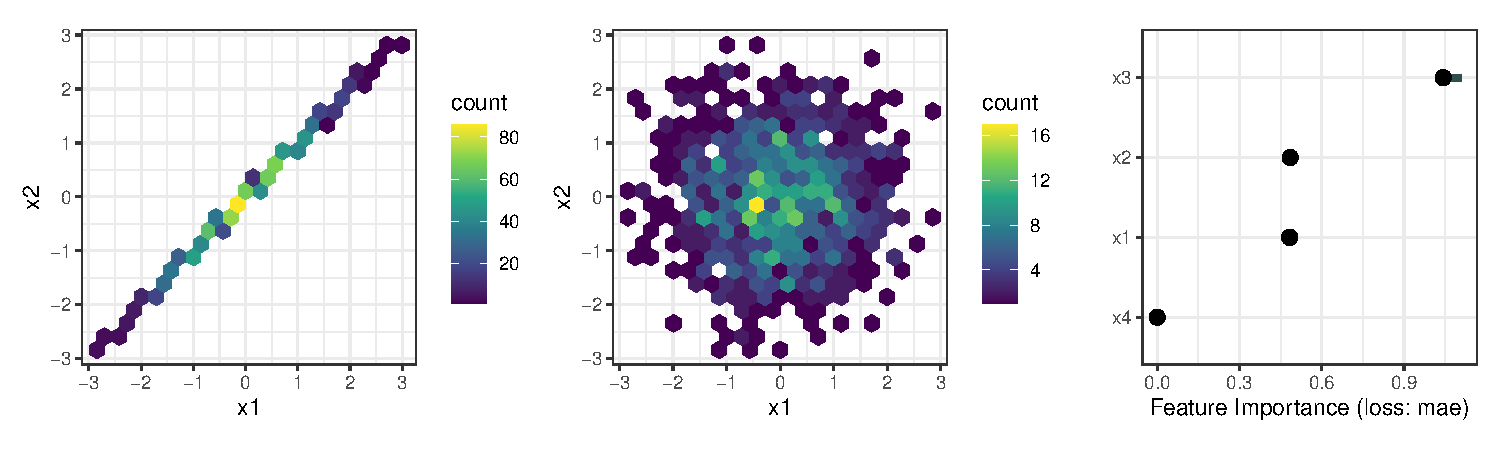
\includegraphics[width=\linewidth]{figure_man/pfi_hexbin_extrapolation.pdf}}

Hexbin plot of $(x_1, x_2)$ before (left) and after (center) permuting $x_1$;  
PFI scores (right).

\begin{itemize}
  \item[$\Rightarrow$] $x_1, x_2$ cancel in $\hat{f}$ since $0.3 x_1 - 0.3 x_2 \approx 0$ and $x_1 \approx x_2$ $\leadsto$ should be irrelevant
  \item[$\Rightarrow$] Permuting $x_1$ breaks joint structure $\leadsto$ unrealistic inputs
  \item[$\Rightarrow$] PFI > 0 due to extrapolation (PFI evaluates model on unrealistic inputs)\\ $\leadsto$ $x_1, x_2$ are misleadingly considered relevant
\end{itemize}

\end{frame}




\begin{frame}{Comments on PFI - Interactions}

\textbf{Example:} Let $x_1, \dots, x_4$ be independently and uniformly sampled from $\{-1, 1\}$ and 
$$y:= x_1 x_2 + x_3 + \epsilon_Y \text{ with } \epsilon_Y \sim N(0, 1)$$

\begin{columns}[T, totalwidth = \textwidth]
\begin{column}{0.5\textwidth}

Fitting a LM yields $\fh(x) \approx x_1 x_2 + x_3$.\\
\lz\pause
Although $x_3$ alone contributes as much to the prediction as $x_1$ and $x_2$ jointly, all three are considered equally relevant.\\
\lz
$\Rightarrow$ PFI does not fairly attribute the performance to the individual features.

\end{column}
\begin{column}{0.5\textwidth}
\centering
  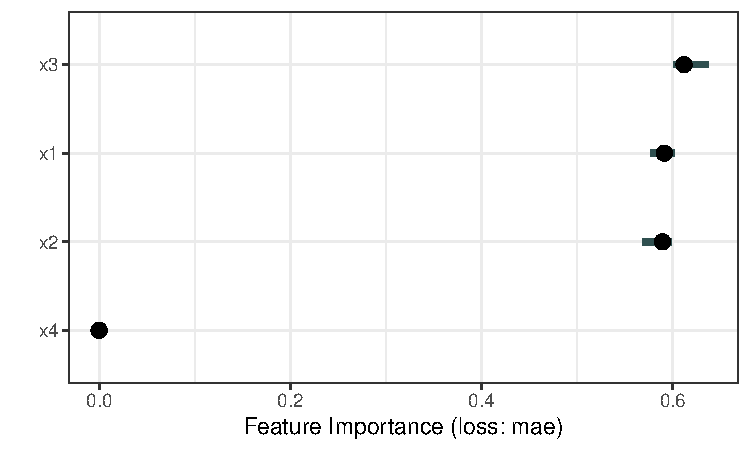
\includegraphics[width=\linewidth]{figure_man/pfi_interactions.pdf}
\end{column}
\end{columns}


\end{frame}

\begin{frame}{Comments on PFI - Test vs. Training data}

\textbf{Example:} $x_1, \dots, x_{20}, y$ are independently sampled from $\mathcal{U} (-10, 10)$. An \texttt{xgboost} model with default hyperparameters is fit on a small training set of $50$ observations. The model overfits heavily.\\

\begin{figure}
  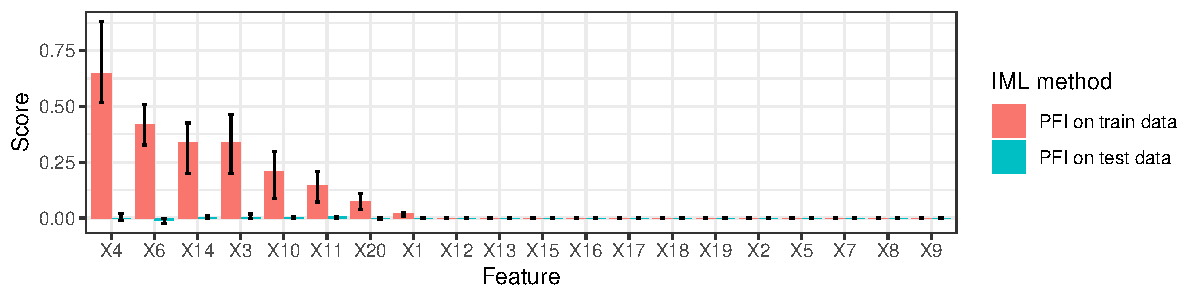
\includegraphics[width=0.9\linewidth]{figure_man/pfi_test_vs_train.pdf}
  \caption{While PFI on test data considers all features to be irrelevant, PFI on train data exposes the features on which the model overfitted.}
\end{figure}

\pause

Why? PFI can only be nonzero if the permutation breaks a dependence in the data. Spurious correlations help the model perform well on train data but are not present in the test data.\\
$\Rightarrow$ If you are interested in which features help the model to generalize, apply PFI on test data.
  
\end{frame}

\begin{frame}{Implications of PFI}

Can we get insight into whether the ...

\begin{enumerate}
    \item<1-> feature $x_j$ is causal for the prediction?
    \begin{itemize}
      \item $PFI_j \neq 0$ $\Rightarrow$ model relies on $x_j$
      %(contraposition does not hold, see training vs. test data example)
      \item As the training vs. test data example demonstrates, the converse does not hold
    \end{itemize}
    \item<2-> feature $x_j$ contains prediction-relevant information?
    \begin{itemize}
      \item $PFI_j \neq 0$  $\Rightarrow$ $x_{j}$ is dependent of $y$ or it's covariates $x_{-j}$ or both (due to extrapolation) 
      \item $x_{j}$ is not exploited by model (regardless of whether it is useful for $y$ or not) $\Rightarrow$ $PFI_j = 0$  %irrespective of whether the feature is useful or not
    \end{itemize}
    \item<3-> model requires access to $x_j$ to achieve it's prediction performance?    
    \begin{itemize}
      \item As the extrapolation example demonstrates, such insight is not possible
\end{itemize}
\end{enumerate}
\end{frame}


% \begin{frame}{Testing Importance (PIMP) \citebutton{Altmann et al. (2010)}{https://doi.org/10.1093/bioinformatics/btq134}}

% \begin{itemize}[<+->]
%   \item PIMP was originally introduced for random forest's built-in permutation feature importance
%   %\item It fixes the problem that the importance measure prefers features with many categories.
%   \item PIMP investigates whether the PFI score \textbf{significantly} differs from 0\\
%   $\Rightarrow$ Useful because PFI can be non-zero due to randomness/stochasticity
%   \item PIMP tests the $H_0$-hypothesis: Feature is independent of the target $y$ (unimportant)
%   %It computes the distribution of importances under the $H_0$-hypothesis that the feature is independent of the target $y$
%   \item Sampling under $H_0$: Permute target $y$, retrain model, compute PFI scores (repeat)\\
%   $\Rightarrow$ Permuting $y$ breaks relationship to all features\\
%   $\Rightarrow$ By computing PFI scores again, we obtain distribution of PFI scores under $H_0$
%   \item %We now rescale the importance to a 
%   Compute p-value - the tail probability under $H_0$ - and use it as a new importance measure
% \end{itemize}

% %\footnote[frame]{\fullcite{altmann2010permutation}}
% %{\tiny{Altmann, André, et al. "Permutation importance: a corrected feature importance measure." 
% %Bioinformatics 26.10 (2010): 1340-134.}}

% \end{frame}

% \begin{frame}{Testing Importance (PIMP)}

% PIMP algorithm:
% \begin{enumerate}
% 	\item<1-3> For $m \in \{1, \ldots, n_{repetitions}\}$:
% 		\begin{itemize}
% 			\item Permute response vector $y$
% 			\item Retrain model with data $\Xmat$ and permuted $y$
% 			\item Compute feature importance $PFI_j^m$ for each feature $j$ (under $H_0$)
% 		\end{itemize}
% 	\item<2-3> Train model with $\Xmat$ and unpermuted $y$
% 	\item<3> For each feature $j \in \{1,\ldots,p\}$:
% 		\begin{itemize}
% 			\item Fit probability distribution of the feature importance values $PFI_j^m$, $m \in \{1, \ldots, n_{repetitions}\}$ (choice between Gaussian, lognormal, gamma or non-parametric)
% 			\item Compute feature importance $PFI_j$ for the model without permutation of $y$ (under $H_1$)
% 			\item Retrieve the p-value of $PFI_j$ based on the fitted distribution
% 		\end{itemize}
% \end{enumerate}
% \end{frame}


% %TODO: Simplify or better explain example
% \begin{frame}{PIMP for extrapolation example}
% \textbf{Recall:} 
% $y = x_3 + \epsilon_y$ with $\epsilon_y \sim N(0, 0.1)$, 
% $x_1$, $x_2$ highly correlated but independent of $y$, 
% $x_4$ is independent of $y$ and all other variables.
% Fitting a LM yields $\fh(\xv) \approx 0.3 x_1 - 0.3 x_2 + x_3$.
% %Fitting a \texttt{lm} yields $\fh(x) \approx 0.3 x_1 - 0.3 x_2 + x_3$.
% %
% %\begin{figure}
%   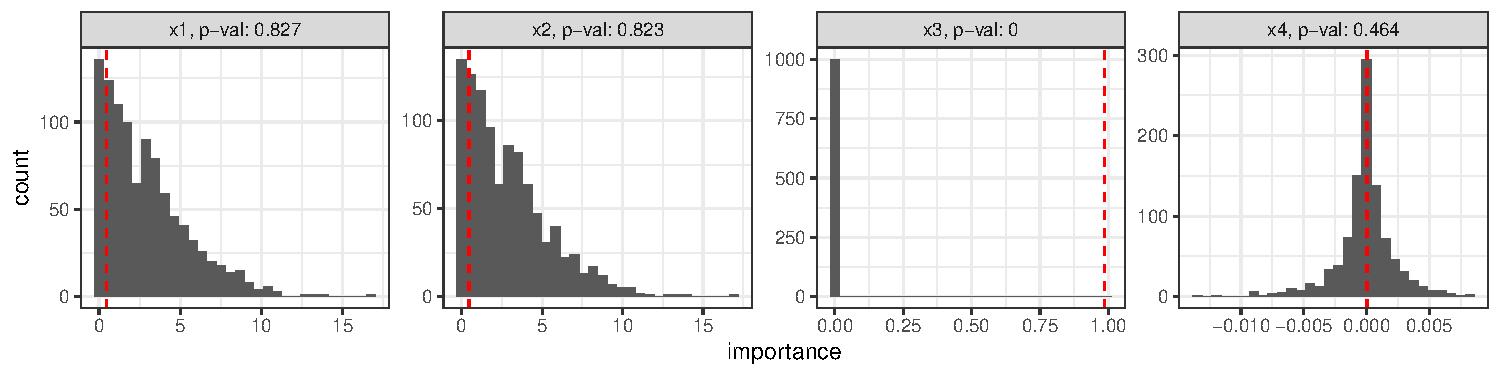
\includegraphics[width=\linewidth]{figure_man/pimp.pdf}
%   %\caption{$H_0$ distribution (1000 samples) for each feature as histograms, the true PFI indicated in red. PIMP only considers $x_3$ relevant. Although PFI for $x_1$ and $x_2$ is nonzero, PIMP considers them irrelevant since they are not predictive of $y$. Even after permuting $y$, the model relies on them.}
% %\end{figure}

% \begin{itemize}
%     \item Histograms: $H_0$ distribution of PFI scores after permuting $y$ (1000 repetitions)
%     \item Red: PFI score estimated on unpermuted $y$ (under $H_1$) $\leadsto$ compare against $H_0$ distribution
%     \item Results: Although PFI for $x_1$ and $x_2$ is nonzero (red), PIMP considers them not significantly relevant (p-value > 0.05) 
%     %since they are not predictive of $y$
% \end{itemize}
% \end{frame}

% \begin{frame}{Digression: Multiple testing problem \citebutton{Romano et al. (2010)}{https://doi.org/10.1057/978-1-349-95121-5_2914-1}}
% \begin{itemize}[<+->]
%   \item When should we reject the $H_0$-hypothesis for a feature? 
%   \item The larger the number of features, the more tests need to be performed by PIMP\\
%   $\leadsto$ \textbf{Multiple testing problem}: If multiplicity of tests is not taken into account, the probability that some of the true $H_0$-hypothesis is rejected (type-I error) by chance may be large
%   \item Accounting for multiplicity of individual tests can be achieved by controlling an appropriate error rate, e.g., the \textbf{family-wise error rate} (FWE: probability of at least one type-I error)
%   \item One classical method to control the FWE is the \textbf{Bonferroni correction} which rejects a null hypothesis if its p-value is smaller than $\alpha/m$ with $m$ as the number of performed parallel tests
%   %\item We refer to other lectures or the statistics literature for more details
%   \end{itemize} 

%   %\footnote[frame]{\fullcite{romano2010multiple}}
%   %{\tiny{Romano, J. P., Shaikh, A. M., and Wolf, M. (2010). Multiple Testing. The New Palgrave Dictionary of Economys. \url{https://home.uchicago.edu/~amshaikh/webfiles/palgrave.pdf}}\par}
% \end{frame}
% % \begin{frame}
% %   \printbibliography
% % \end{frame}

\endlecture
\end{document}
